\documentclass[prb,preprint]{revtex4-1} 
% The line above defines the type of LaTeX document.
% Note that AJP uses the same style as Phys. Rev. B (prb).

\usepackage{amsmath}  % needed for \tfrac, \bmatrix, etc.
\usepackage{amsfonts} % needed for bold Greek, Fraktur, and blackboard bold
\usepackage{graphicx} % needed for figures
\usepackage{color}
\usepackage{ulem}
\usepackage{multirow}
\begin{document}

% Be sure to use the \title, \author, \affiliation, and \abstract macros
% to format your title page.  Don't use lower-level macros to  manually
% adjust the fonts and centering.

\title{Single-Photon Interference}


\author{Liza Mulder}
\email{emulder@smith.edu}
\affiliation{Department of Physics, Smith College, Northampton, MA 01063}


\author{Frances Yang}
\email{fyang@smith.edu}
\affiliation{Department of Physics, Smith College, Northampton, MA 01063}


\date{\today}



\begin{abstract}

\end{abstract}

\maketitle

\section{Introduction} 

The Franck-Hertz Experiment is named for James Franck and Gustav Hertz, who used it to demonstrate discrete energy levels in atoms. 
They received the Nobel Prize in 1925 for their work on this experiment. 
In the experiment a beam of electrons is sent through a cloud of atoms, usually mercury or neon. 
Atoms can only gain energy in an amount equal to an allowed transition between energy levels. 
Only electrons with energies equal to these transition energies can transfer their energy to an atom. 
Electrons that have too much or too little energy will collide elastically with the atoms, keeping their energy. 
We then measure the current of electrons leaving the gas - fewer reach the detector when they transfer energy to atoms in collisions. 
This causes dips in the current whose spacing is related to the transition energies. 
In this way the Franck-Hertz experiment can be used to determine the transition energies of the atom. 

\section{Methods}

For this experiment we used a Franck-Hertz experimental apparatus from ELWE. A diagram is shown in Figure ~\ref{set-up}. 
A filament with 120 mA of current creates a cloud of electrons. 
A potential difference (which we call the accelerating voltage) drives the electrons through a gas of mercury atoms. 
We can control the energy of the electrons by varying the accelerating voltage. 
Electrons which have transferred energy in collisions have less energy at the other end of the apparatus. 
A retarding potential prevents these electrons from reaching the anode. 
The current at the anode was converted to a voltage by the apparatus. 
To take data, we slowly increased the accelerating voltage from zero until the gas began to ionize, and measured the output voltage from the anode. 


\begin{figure}[h!]
\centering
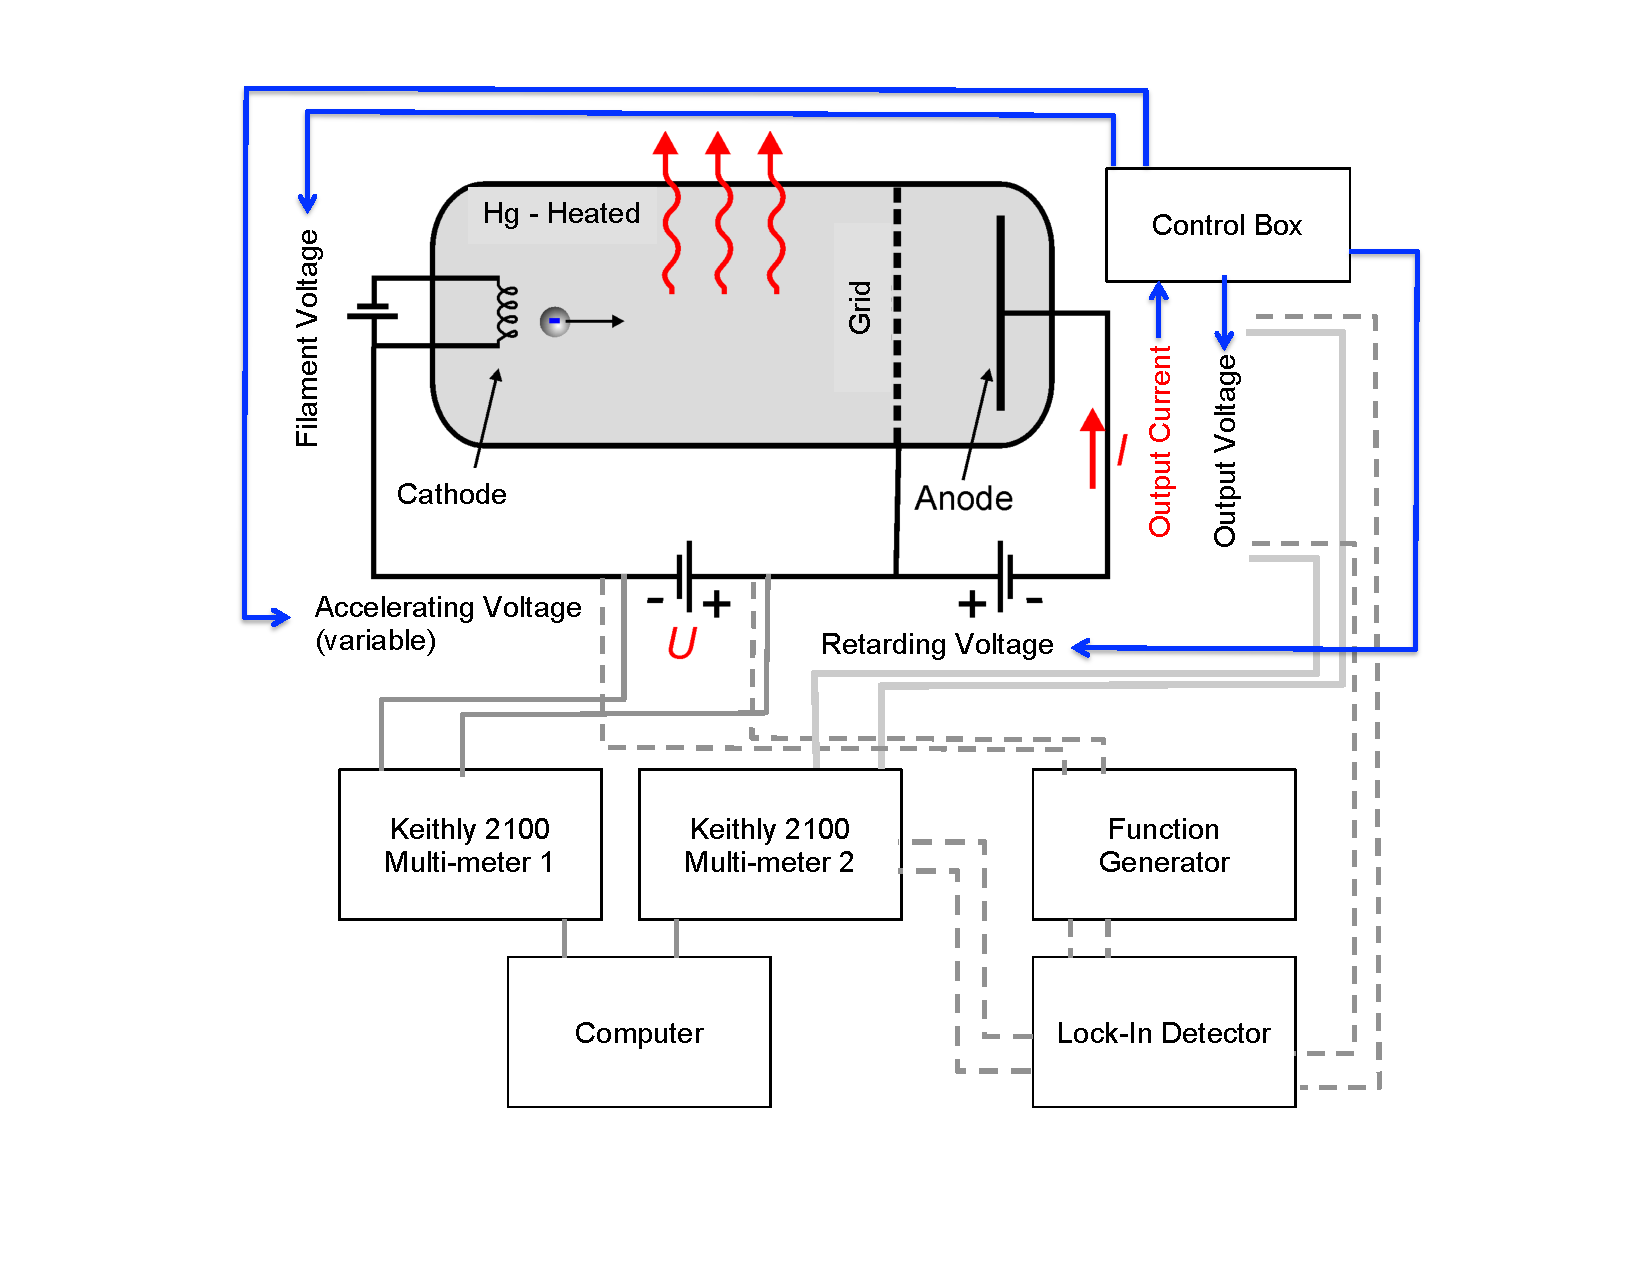
\includegraphics[width=5in]{set-up.pdf}
\caption{The ELWE experimental apparatus, with the connections used to take measurements using both the direct method and the lock-in method. The apparatus consists of a control box (supplying the filament voltage, accelerating voltage, retarding voltage, and output voltage) and an oven, inside of which is the cloud of heated gas, the filament, the grid, and the anode. The filament releases a cloud of electrons into the gas, the grid supplies the positive voltage to attract the electrons, the anode collects the electrons, and the resulting current is measured as a voltage in the control box. The temperature of the oven, the accelerating voltage (applied between the cathode and the grid), the filament voltage, and the retarding voltage can be varied. For direct measurements, we sent the accelerating voltage from the control box to one multi-meter, and the output voltage to another, and the measurements from the multi-meters went to the computer (solid gray lines).  To use the lock-in (dark gray connections, dashed and solid), we supplied an oscillating voltage from the function generator on top of the accelerating voltage supplied by the control box. The output voltage and the reference from the function generator both went to the lock-in detector, and from there to the second multi-meter and then the computer. }
\label{set-up}
\end{figure}

\section{Results}

\section{Analysis}

\begin{table}[h!]
\centering
\caption{ }
\begin{ruledtabular}
\begin{tabular}{lc}
     
\end{tabular}
\end{ruledtabular}
\label{parameters}
\end{table}


\section{Discussion}


\section{Conclusion}

\begin{thebibliography}{3}

\end{thebibliography}
\end{document}
